\documentclass[a4paper,twoside,12pt]{article}
\usepackage{graphicx}

\newcommand{\noun}[1]{\textsc{#1}}

\usepackage{verbatim}
\newenvironment{metaverbatim}{\verbatim}{\endverbatim}


\begin{document}
%	\fontfamily{phv}		% Did not work as intended
\begin{titlepage}	
	\title{\noun{Worksheet 2\\ Version Control Systems}}

	\author{\textsc{Team 2}\\ Abela Tharen, Camilleri Daniel, Farrugia Gabriel, Schembri Matthew\\	University of Malta}
	% Align Properly with Center OR Under \title
	\date{}
	
	\maketitle
	\tableofcontents
\end{titlepage}	

\pagebreak

\section{Git Repository Details}
\paragraph{GitHub was used to manage the online repository, and through which the task was handled.}
\subsection{Git Repository Resource Links}
\paragraph{GitHub Page URL\\ \texttt{https://github.com/danielsna/team-2/archive/master.zip}}
\paragraph{Clone with HTTPS\\ \texttt{https://github.com/danielsna/team-2.git}}
\paragraph{Download ZIP Archive\\ \texttt{https://github.com/danielsna/team-2/archive/master.zip}}

\pagebreak[2]
\section{Version Control Terminology}
\subsection{Repository Content}
\begin{center}
	\renewcommand{\arraystretch}{1.25}
	\begin{tabular}{ | l | p{7.5cm} |}
		\hline
		File/Directory/Tag & Description \\ \hline
		\texttt{Ingredients.txt} & Where all ingredients were compiled and stored \\ \hline
		\texttt{Recipe\_Book.txt} & Where all recipes and ingredients were compiled and stored. \\ \hline
		TAG \texttt{Recipe\_Book\_Draft\_1} & All ingredients and recipes were pushed. \\ \hline
		TAG \texttt{Recipe\_Book\_Draft\_2} & All ingredients and recipes were pushed in an orderly fashion. \\ \hline
		\texttt{Recipe\_Book\_Drafts}\textbackslash & Each recipe was  stored within as a text draft, later compiled within \texttt{Recipe\_Book.txt} \\ \hline
		\texttt{Screenshots}\textbackslash & Screenshots of all merge conflicts were stored here \\ \hline
	\end{tabular}
\end{center}

\begin{comment}
\subsection{Making use of GitHub Front-End Functionality}
\paragraph{GitHub offers extra features, which were explored to further aid development of the assignment}
\subsubsection{Using Markdown for \texttt{README}}
\paragraph{The Markdown Integration built in GitHub, allowed for features, most significantly Tables \& Task Lists, that helped in defining the objectives required to complete the assignment}
\subsubsection{Using Issues to Resolve Obstacles}
\paragraph{Issues were used to put forward problems that came about, while using Git. Issues opened included the requirement for team members and difficulties in creating a merge conflict.}
\end{comment}

\pagebreak[4]
\section{Merge Conflicts during Development}
\begin{figure}[ht!]
	\centering
	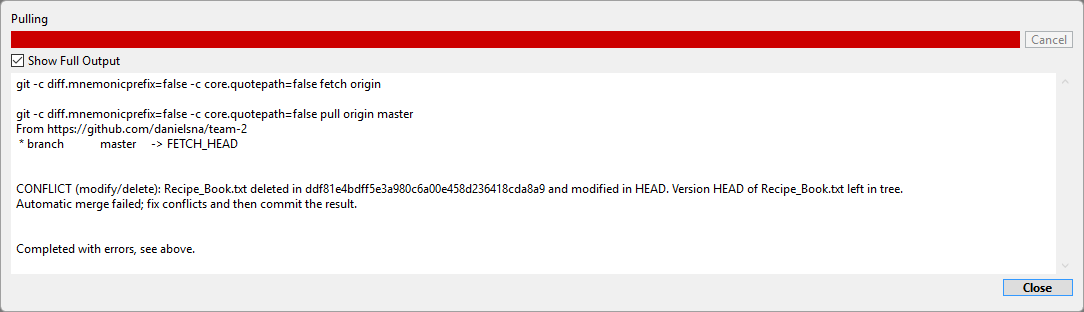
\includegraphics[width=145mm]{Merge_Conflict_001.png}
	\caption{Merge Conflict when pushing to existing \texttt{Recipe\_Book.txt}}
\end{figure}
\begin{figure}[ht!]
	\centering
	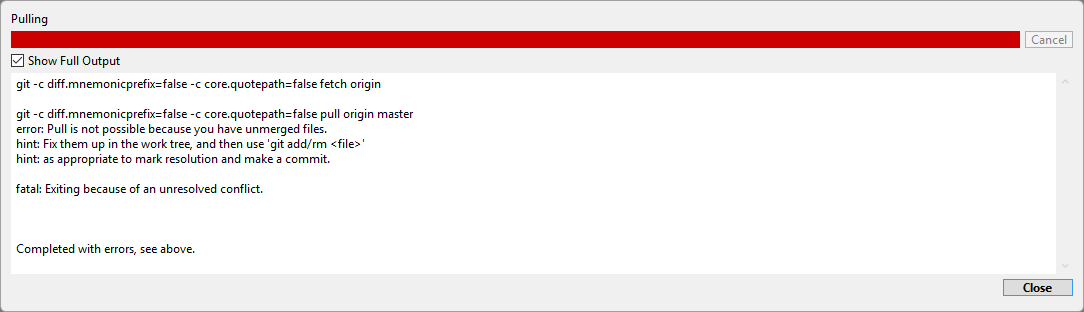
\includegraphics[width=145mm]{Merge_Conflict_002.png}
	\caption{Merge Conflict when pulling from repository}
\end{figure}
\begin{figure}[ht!]
	\centering
	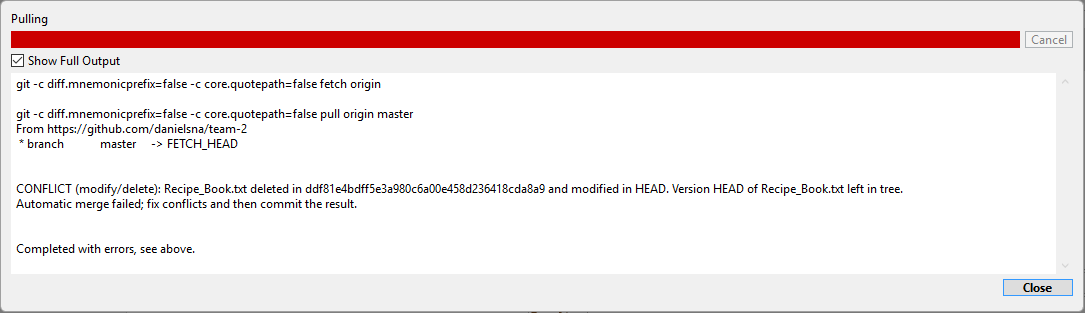
\includegraphics[width=145mm]{Merge_Conflict_003.png}
	\caption{Merge Conflict as \texttt{Recipe\_Book.txt} could not merge automatically}
\end{figure}
% Make Last Figure and Caption Align Properly with Center

\pagebreak[4]
\section{\LaTeX\ Source Code}

\begin{verbatim}
\documentclass[a4paper,twoside,12pt]{article}
\usepackage{graphicx}

\newcommand{\noun}[1]{\textsc{#1}}

\usepackage{verbatim}
\newenvironment{metaverbatim}{\verbatim}{\endverbatim}


\begin{document}
%	\fontfamily{phv}		% Did not work as intended
\begin{titlepage}	
\title{\noun{Worksheet 2\\ Version Control Systems}}

\author{\textsc{Team 2}\\ Abela Tharen, Camilleri Daniel, 
Farrugia Gabriel, Schembri Matthew\\	University of Malta}

\date{}

\maketitle
\tableofcontents
\end{titlepage}	

\pagebreak

\section{Git Repository Details}
\paragraph{GitHub was used to manage the online repository, and through 
which the task was handled.}
\subsection{Git Repository Resource Links}
\paragraph{GitHub Page URL\\ 
\texttt{https://github.com/danielsna/team-2/archive/master.zip}}
\paragraph{Clone with HTTPS\\ 
\texttt{https://github.com/danielsna/team-2.git}}
\paragraph{Download ZIP Archive\\ 
\texttt{https://github.com/danielsna/team-2/archive/master.zip}}

\pagebreak[2]
\section{Version Control Terminology}
\subsection{Repository Content}
\begin{center}
\renewcommand{\arraystretch}{1.25}
\begin{tabular}{ | l | p{7.5cm} |}
\hline
File/Directory/Tag & Description \\ \hline
\texttt{Ingredients.txt} & Where all ingredients were compiled and stored 
\\ \hline
\texttt{Recipe\_Book.txt} & Where all recipes and ingredients were compiled 
and stored. \\ \hline
TAG \texttt{Recipe\_Book\_Draft\_1} & All ingredients and recipes were 
pushed. \\ \hline
TAG \texttt{Recipe\_Book\_Draft\_2} & All ingredients and recipes were 
pushed in an orderly fashion. \\ \hline
\texttt{Recipe\_Book\_Drafts}\textbackslash & Each recipe was  stored 
within as a text draft, later compiled within \texttt{Recipe\_Book.txt} \\ 
\hline
\texttt{Screenshots}\textbackslash & Screenshots of all merge conflicts 
were stored here \\ \hline
\end{tabular}
\end{center}

\begin{comment}
\subsection{Making use of GitHub Front-End Functionality}
\paragraph{GitHub offers extra features, which were explored to further aid 
development of the assignment}
\subsubsection{Using Markdown for \texttt{README}}
\paragraph{The Markdown Integration built in GitHub, allowed for features, 
most significantly Tables \& Task Lists, that helped in defining the 
objectives required to complete the assignment}
\subsubsection{Using Issues to Resolve Obstacles}
\paragraph{Issues were used to put forward problems that came about, while 
using Git. Issues opened included the requirement for team members and 
difficulties in creating a merge conflict.}
\end{comment}

\pagebreak[4]
\section{Merge Conflicts during Development}
\begin{figure}[ht!]
\centering
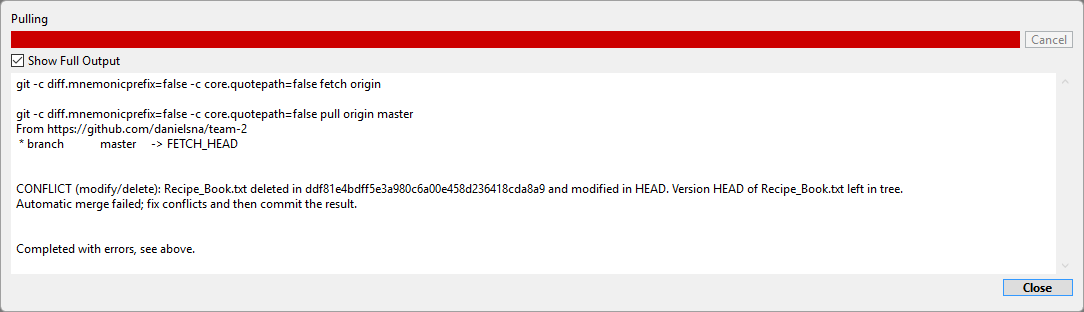
\includegraphics[width=145mm]{Merge_Conflict_001.png}
\caption{Merge Conflict when pushing to existing \texttt{Recipe\_Book.txt}}
\end{figure}
\begin{figure}[ht!]
\centering
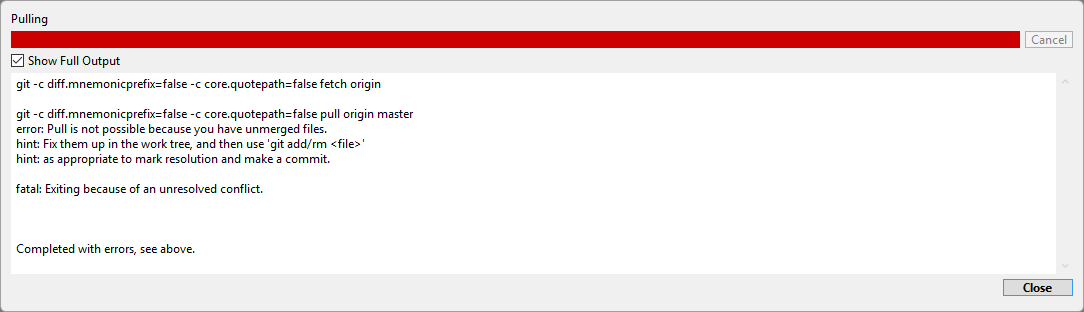
\includegraphics[width=145mm]{Merge_Conflict_002.png}
\caption{Merge Conflict when pulling from repository}
\end{figure}
\begin{figure}[ht!]
\centering
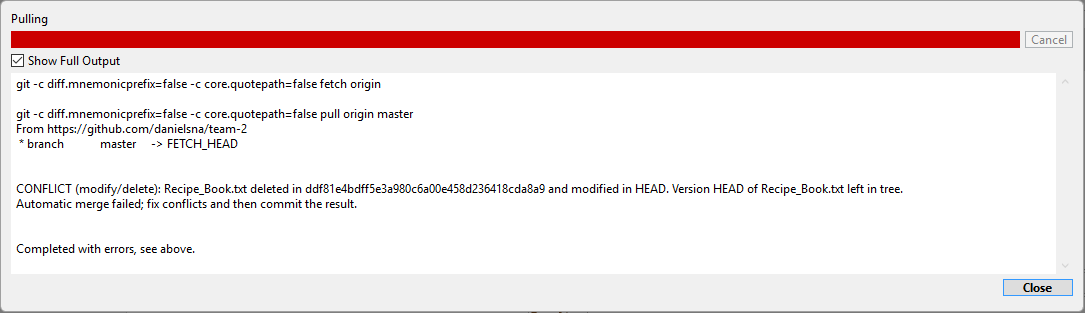
\includegraphics[width=145mm]{Merge_Conflict_003.png}
\caption{Merge Conflict as \texttt{Recipe\_Book.txt} could not merge 
automatically}
\end{figure}


\pagebreak[4]
\section{\LaTeX\ Source Code}
\end{verbatim}
	\par\noindent\texttt{\textbackslash begin\{verbatim\}}\\*
	\indent\LaTeX{} Source Code
	\par\noindent\texttt{\textbackslash end\{verbatim\} }
\begin{verbatim}
	\end{document}
\end{verbatim}

\end{document}
